\documentclass{article}

\usepackage{graphicx}
\usepackage{tikz}
\usepackage{tikzsymbols}
\usetikzlibrary{calc,patterns,shapes.geometric}
\pagestyle{empty}
\usepackage[margin=0pt]{geometry}
\geometry{papersize={14in,12in}}

\def\centerarc[#1](#2)(#3:#4:#5){\draw[#1] ($(#2)+({#5*cos(#3)},{#5*sin(#3)})$) arc (#3:#4:#5);}

\begin{document}
	\begin{figure}
		\centering
		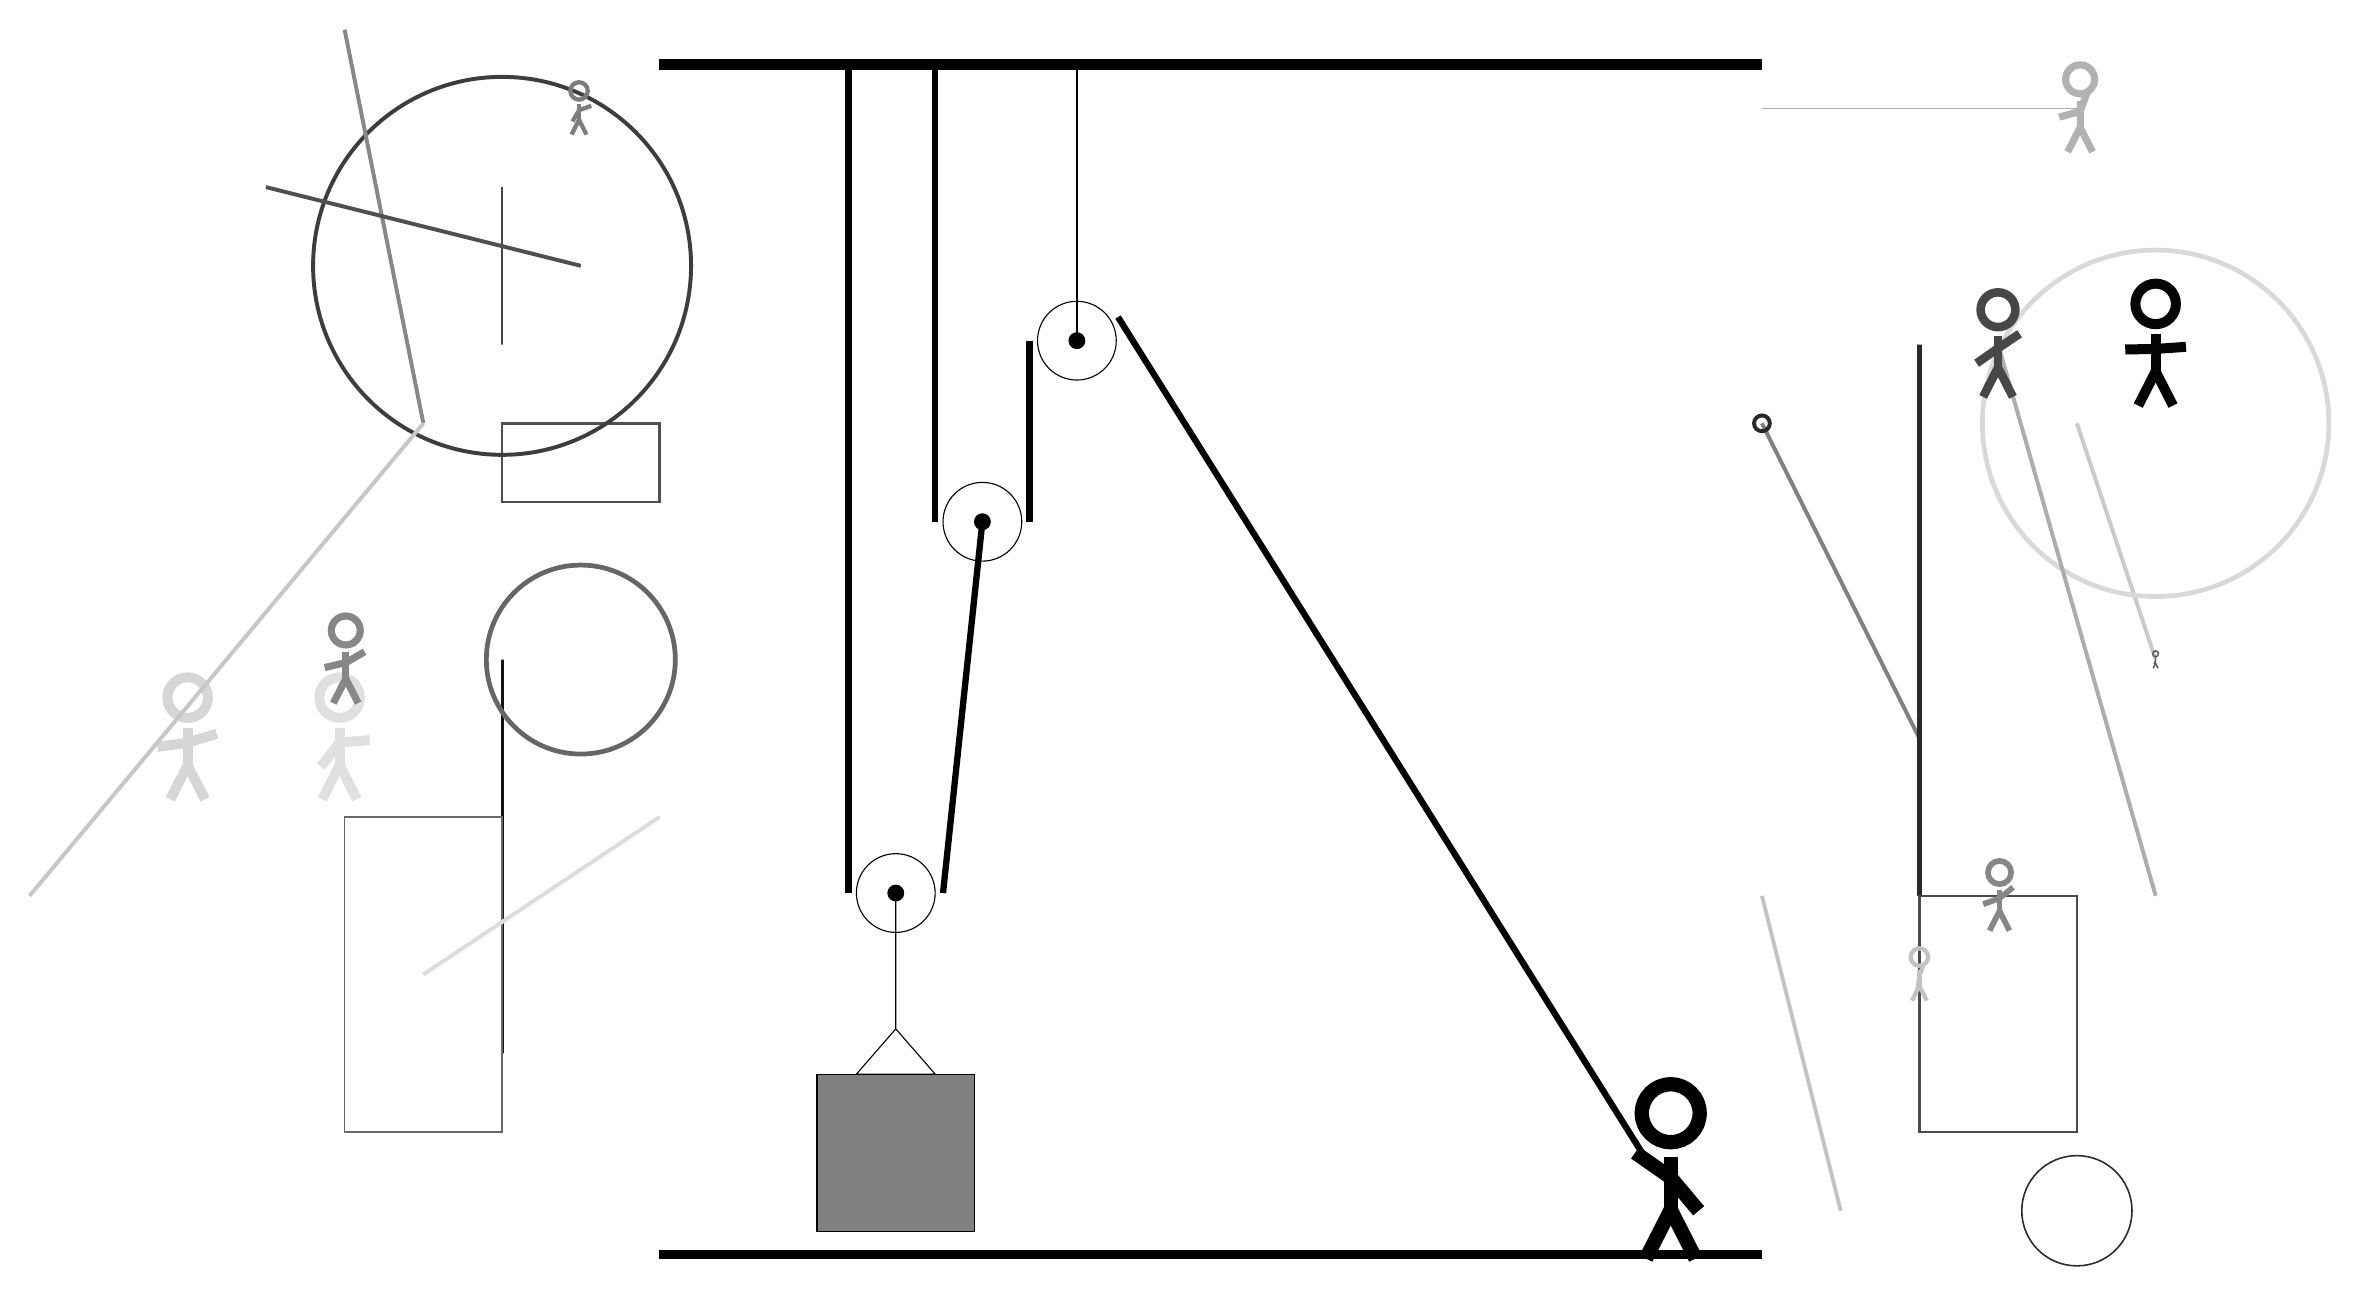
\begin{tikzpicture}
			%%%%% START %%%%%
			
			\draw[fill=black] (-2, 11.5) rectangle (12, 11.625);
			
			\draw (1, 1.035) circle (0.5);
			\draw[fill=black] (1, 1.035) circle (0.1);
			
			\draw (2.1, 5.75) circle (0.5);
			\draw[fill=black] (2.1, 5.75) circle (0.1);
			
			\draw (3.3, 8.05) circle (0.5);
			\draw[fill=black] (3.3, 8.05) circle (0.1);
			\draw[thick] (3.3, 8.05) -- (3.3, 11.5);
			
			\draw (1, 1.035) -- (1, -0.69) -- (0.5, -1.265) -- (1.5, -1.265) -- (1, -0.69);
			\draw[fill=black!50] (0, -1.265) rectangle (2, -3.265);
			
			\draw[line width=0.5mm, color=black!50](14, 3) -- (12, 7);
			
			\draw[line width=0.2mm, color=black!32] (12, 11) rectangle (16, 11);
			\draw[line width=0.5mm, color=black!21](17, 4) -- (16, 7);
			\draw [line width=0.2mm, color=black!83](16, -3) circle (0.7);
			
			\draw[line width=0.4mm, color=black!93] (-4, -1) rectangle (-4, 4);
			\draw [line width=0.6mm, color=black!15](17, 7) circle (2.2);
			\node[line width=0.6mm, color=black!98] at (17, 8) {\Strichmaxerl[7][1][4]};
			\draw[line width=0.3mm, color=black!69] (-4, 7) rectangle (-2, 6);
			\draw[line width=0.7mm, color=black!84] (14, 1) rectangle (14, 8);
			\node[line width=0.5mm, color=black!66] at (17, 4) {\Strichmaxerl[1][71][90]};
			\node[line width=0.3mm, color=black!12] at (-6, 3) {\Strichmaxerl[7][52][5]};
			\draw[line width=0.5mm, color=black!32](17, 1) -- (15, 8);
			\node[line width=0.7mm, color=black!16] at (-8, 3) {\Strichmaxerl[7][8][17]};
			
			\draw [line width=0.5mm, color=black!84](12, 7) circle (0.1);
			\draw[line width=0.2mm, color=black!59] (-4, 2) rectangle (-6, -2);
			\draw [line width=0.5mm, color=black!76](-4, 9) circle (2.4);
			\node[line width=0.3mm, color=black!30] at (16, 11) {\Strichmaxerl[5][15][70]};
			
			\draw [line width=0.6mm, color=black!60](-3, 4) circle (1.2);
			\draw[line width=0.5mm, color=black!23](12, 1) -- (13, -3);
			\draw[line width=0.3mm, color=black!70] (14, 1) rectangle (16, -2);
			\node[line width=0.6mm, color=black!47] at (15, 1) {\Strichmaxerl[4][20][39]};
			
			\draw[line width=0.3mm, color=black!72] (-4, 8) rectangle (-4, 10);
			\node[line width=0.7mm, color=black!24] at (14, 0) {\Strichmaxerl[3][82][71]};
			\node[line width=0.6mm, color=black!47] at (-6, 4) {\Strichmaxerl[5][13][30]};
			\draw[line width=0.5mm, color=black!47](-6, 12) -- (-5, 7);
			
			\draw[line width=0.5mm, color=black!69](-7, 10) -- (-3, 9);
			\draw[line width=0.5mm, color=black!22](-5, 7) -- (-10, 1);
			\node[line width=0.2mm, color=black!72] at (15, 8) {\Strichmaxerl[6][35][34]};
			\draw[line width=0.5mm, color=black!13](-5, 0) -- (-2, 2);
			
			\node[line width=0.5mm, color=black!51] at (-3, 11) {\Strichmaxerl[3][60][20]};
			
			\draw[line width=0.8mm] (0.4, 11.5) -- (0.4, 1.035);
			\centerarc[line width=0.8mm](1, 1.035)(180:360:0.6);
			\draw[line width=0.8mm](1.6, 1.035) -- (2.1, 5.75);
			\draw[line width=0.8mm] (1.5, 11.5) -- (1.5, 5.75);
			\centerarc[line width=0.8mm](2.1, 5.75)(180:360:0.6);
			\draw[line width=0.8mm](2.7, 5.75) -- (2.7, 8.05);
			\centerarc[line width=0.8mm](3.3, 8.05)(30:180:0.6);
			\draw[line width=0.8mm] (3.822, 8.35) -- (10.5, -2.3);
			
			\node at (10.8, -2.5) {\Strichmaxerl[10][-35][-50]};
			
			\draw[fill=black] (-2, -3.5) rectangle (12, -3.6);
			
			%%%%% END %%%%%
		\end{tikzpicture}
	\end{figure}	
\end{document}